\documentclass[tikz,border=2pt]{standalone}
\usepackage{amsmath}
\usepackage{pgfplots}
\pgfplotsset{compat=1.18}
\usetikzlibrary{arrows.meta}
\begin{document}
% Battle of the Sexes, p = sigma_1(O), q = sigma_2(O). BR_1: p = 0 for q < 1/3, any p at q = 1/3,
% p = 1 for q > 1/3. BR_2: q = 0 for p < 2/3, any q at p = 2/3, q = 1 for p > 2/3.
% They cross at (0,0) = (F,F), (1,1) = (O,O) and the mixed equilibrium (2/3, 1/3).
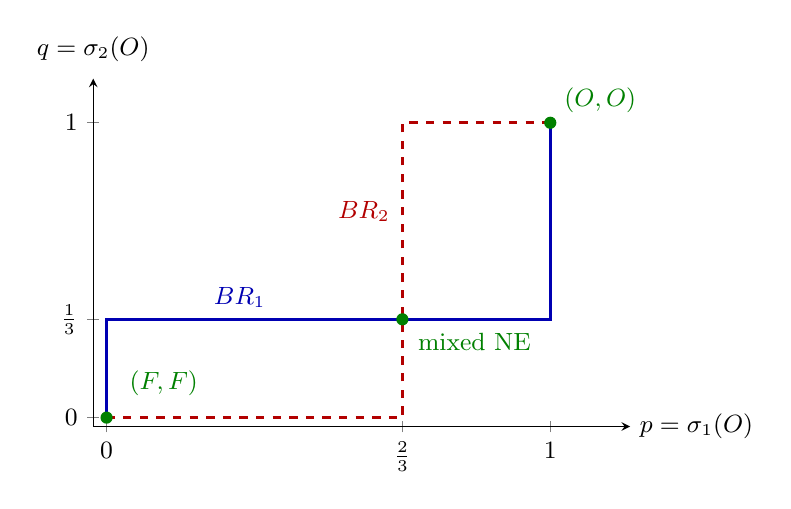
\begin{tikzpicture}[font=\small, >={Latex[length=2mm]}]
  \begin{axis}[
    axis lines=left, xmin=-0.03, xmax=1.18, ymin=-0.03, ymax=1.15,
    xtick={0,0.6667,1}, xticklabels={$0$,$\tfrac23$,$1$},
    ytick={0,0.3333,1}, yticklabels={$0$,$\tfrac13$,$1$},
    xlabel={$p=\sigma_1(O)$}, ylabel={$q=\sigma_2(O)$},
    xlabel style={anchor=west, at={(axis description cs:1.0,0.0)}},
    ylabel style={rotate=-90, anchor=south, at={(axis description cs:0,1.02)}},
    width=8.4cm, height=6cm, clip=false]
    % BR_1 (player 1, blue, solid)
    \addplot[blue!70!black, very thick] coordinates {(0,0) (0,0.3333) (1,0.3333) (1,1)};
    % BR_2 (player 2, red, dashed)
    \addplot[red!70!black, very thick, dashed] coordinates {(0,0) (0.6667,0) (0.6667,1) (1,1)};
    \node[blue!70!black, anchor=south] at (axis cs:0.3,0.34) {$BR_1$};
    \node[red!70!black, anchor=east] at (axis cs:0.66,0.7) {$BR_2$};
    % equilibria
    \fill[green!50!black] (axis cs:0,0) circle (2.2pt);
    \fill[green!50!black] (axis cs:1,1) circle (2.2pt);
    \fill[green!50!black] (axis cs:0.6667,0.3333) circle (2.2pt);
    \node[green!50!black, anchor=south west] at (axis cs:0.03,0.04) {$(F,F)$};
    \node[green!50!black, anchor=south west] at (axis cs:1.01,1.0) {$(O,O)$};
    \node[green!50!black, anchor=north west] at (axis cs:0.68,0.32) {mixed NE};
  \end{axis}
\end{tikzpicture}
\end{document}
